
The $\Wjets$ and ${\rm QCD}$ multijet backgrounds are estimated from a sample
of events in which one lepton passes the nominal requirements while
the other passes a looser set of requirements but which fails the
nominal ones.  The looser requirements are defined by looser criteria on
impact parameter and isolation.
This sample, enriched in $\Wjets$ events,
is extrapolated to the signal region using the efficiencies for such
loosely-identified fake leptons to pass the tight selection. These efficiencies
are measured in data using multi-jet events and are parametrized according
to the kinematics of the lepton candidate. 
The systematic uncertainty is about $36\%$, coming mainly from the
estimation of these efficiencies.

The normalization of the top background that survives the top veto
is estimated from data by
counting top~tagged events, $N_{\rm tagged}$. The background from
mis-tagged non~top events, $N_{\rm tagged}^{\rm bkg}$, is subtracted,
and the corresponding event top tagging efficiency is applied.
The event top tagging efficiency, $\epsilon_{\rm top~tagged}$, is measured in a 
data control sample dominated by $\ttbar$ and tW events, selected by
requiring one b-tagged jet with $\Et > 30$~\GeV. The background from mis-tagged non~top events
is subtracted from both the numerator and denominator. 
The top background, $N_{\rm not~tagged}$, is then given by
%
\begin{eqnarray*}
N_{\rm not~tagged} = (N_{\rm tagged} - N_{\rm tagged}^{\rm bkg}) \times (1-\epsilon_{\rm top~tagged})/\epsilon_{\rm top~tagged},
\label{eq:topest}
\end{eqnarray*}

The systematic uncertainty on $N_{\rm not~tagged}$
is about $18\%$, which is dominated by the statistical uncertainty in the
control sample and from systematic uncertainties related to the measurement
of $\epsilon_\text{top tagged}$.

% -- old --
%The residual $\Z/\GAMMA^*$ boson contribution to the $\Elp\Elm$ and $\Mp\Mm$ 
%final states is based on extrapolation from the observed number of events with 
%a dilepton mass within $\pm$~7.5~$\GeVcc$ of the $\Z$ mass, where the residual
%background is subtracted as estimated from $\Elpm\Mmp$ events. The extrapolation 
%to the signal region is done using the simulation and the results are cross-checked 
%in data. The largest uncertainty on the estimate is related to the statistical
%uncertainty of the control sample yield.
% ----

We estimate the Drell-Yan contribution to the $\Elp\Elm$ and
$\Mp\Mm$ final states outside of the Z mass window
$N_{\rm out}^{\ell\ell,{\rm exp}}$, by normalising the 
simulation to the observed number of events inside the $\Z$ mass window, 
$N_{\rm in}^{\ell\ell}$, after subtracting non Drell-Yan backgrounds. 
The backgrounds from $t\bar{t}$, $\WW$, and $\WZ$ and $\ZZ$ events where both
leptons do not come from the same $\rm Z$ boson, $N_{\rm in}^{\rm{non-Z}}$,
are subtracted by counting the number of $\Elpm\Mmp$ events in the Z mass window, 
taking into account combinatorics and 
the relative detection efficiencies for electrons and muons.
The $\WZ$ and $\ZZ$ background, $N_{\rm in}^{\rm ZV}$, 
where both leptons come from the same 
${\rm Z}$ boson, is subtracted by using simulation. 
The residual Drell-Yan background in data outside the Z mass window is thus expressed as
%
\begin{eqnarray*}
N_{\rm out}^{\ell\ell,{\rm exp}} = R^{\ell\ell}_{\rm out/in}\left(N_{\rm in}^{\ell\ell} - N_{\rm in}^{\rm{non-Z}} - N_{\rm in}^{ZV}\right),
~\mathrm{with}~R^{\ell\ell}_{\rm out/in} = N_{\rm out}^{\ell\ell,{\rm MC}}/N_{\rm in}^{\ell\ell,{\rm MC}}.
\label{eq:dyest}
\end{eqnarray*}

The systematic uncertainty on the final estimate is derived from the dependence
of $R^{\ell\ell}_{\rm out/in}$ on the value of the $\met$ cut, by taking
the difference between the $R^{\ell\ell}_{\rm out/in}$ value in the signal region and in a
region where the $\met$ cut has been relaxed.
The value of the systematic uncertainty is $24\%$.

% --Dave-- 
%The $\dytt$ contamination is estimated using $\dyee$ and $\dymm$
%events selected in data, where the leptons are replaced with simulated
%$\Tau$ decays, thus providing a better description of the experimental conditions
%with respect to the simulation.

Finally, a control sample with three reconstructed leptons is used to measure the 
cross section of the $\wgamma^{*}$ process. 
We only use $\wgamma^{*} \rightarrow \ell\nu\Mp\Mm$ events 
for this measurement because the $\ell\nu\Elp\Elm$ final state is difficult to
separate from other backgrounds. Therefore the pair of oppositely charged
leptons with the lowest invariant mass must be a pair of muons. This
measurement is used to normalise the simulated $\wgamma^{*}$ background
contribution from asymmetric gamma decays, in which one lepton escapes
detection~\cite{wgammastart}.

Other backgrounds, such as the $\WZ$ and $\ZZ$ diboson production, are estimated
from simulation. The  $\Wjets$ and $\wgamma$/$\wgamma^{*}$ background
estimate is cross-checked in data using the events passing all the selection
requirements, except that the two leptons must have the same charge; this sample
is dominated by $\Wjets$ and $\wgamma$/ $\wgamma^{*}$ events, after subtracting the expected
$\WZ$ background, where one lepton from the $\Z$ decay is lost.
The  $\dytt$ contamination is
also cross-checked using $\dyee$ and $\dymm$ events selected in data, where the
leptons are replaced with simulated $\Tau$ decays, showing good agreement with expectation from simulation.

The estimated event yields from all processes after applying the event selection are summarized in 
Table~\ref{tab:wwselection_all}, where the WW contributions are calculated assuming the
SM cross section. The distributions of the key analysis variables are 
shown in Figure~\ref{fig:distributions}, where the WW contribution is normalized
according to the measured cross section.

\begin{table}[!h]
  \begin{center}
    \caption{Observed and expected event yields in $\usedLumi$. The prediction 
    for the $\WW$ process assumes the SM cross section value.
    \label{tab:wwselection_all}}
   \begin{tabular}{l|c}
        \hline
        sample                  & yield   $\pm$ stat. $\pm$ syst. \\ \hline
        gg$\to$WW               &   $43.3  \pm  1.0  \pm 13.4$    \\
        qq$\to$WW               &  $640.3  \pm  4.9  \pm 47.4$    \\ \hline
        \ttbar + tW             &  $131.6  \pm 12.7  \pm 19.5$    \\
        W + jets                &   $60.0  \pm  4.3  \pm 21.6$    \\
        WZ + ZZ                 &   $27.4  \pm  0.5  \pm  2.9$    \\
        Z$/\gamma^*$            &   $42.5  \pm  6.0  \pm  9.9$    \\
	W$\gamma$ + W$\gamma^*$ &   $13.6  \pm  2.4  \pm  4.3$    \\
        total background        &  $275.2  \pm 14.9  \pm 31.2$    \\ \hline
        signal + background     &  $958.8  \pm 15.7  \pm 58.3$    \\ \hline
        data                    & $1111    \pm 33$                \\ \hline
      \end{tabular}
  \end{center}
\end{table}

\begin{figure}[h!]
\begin{center}
\begin{tabular}{cc}
  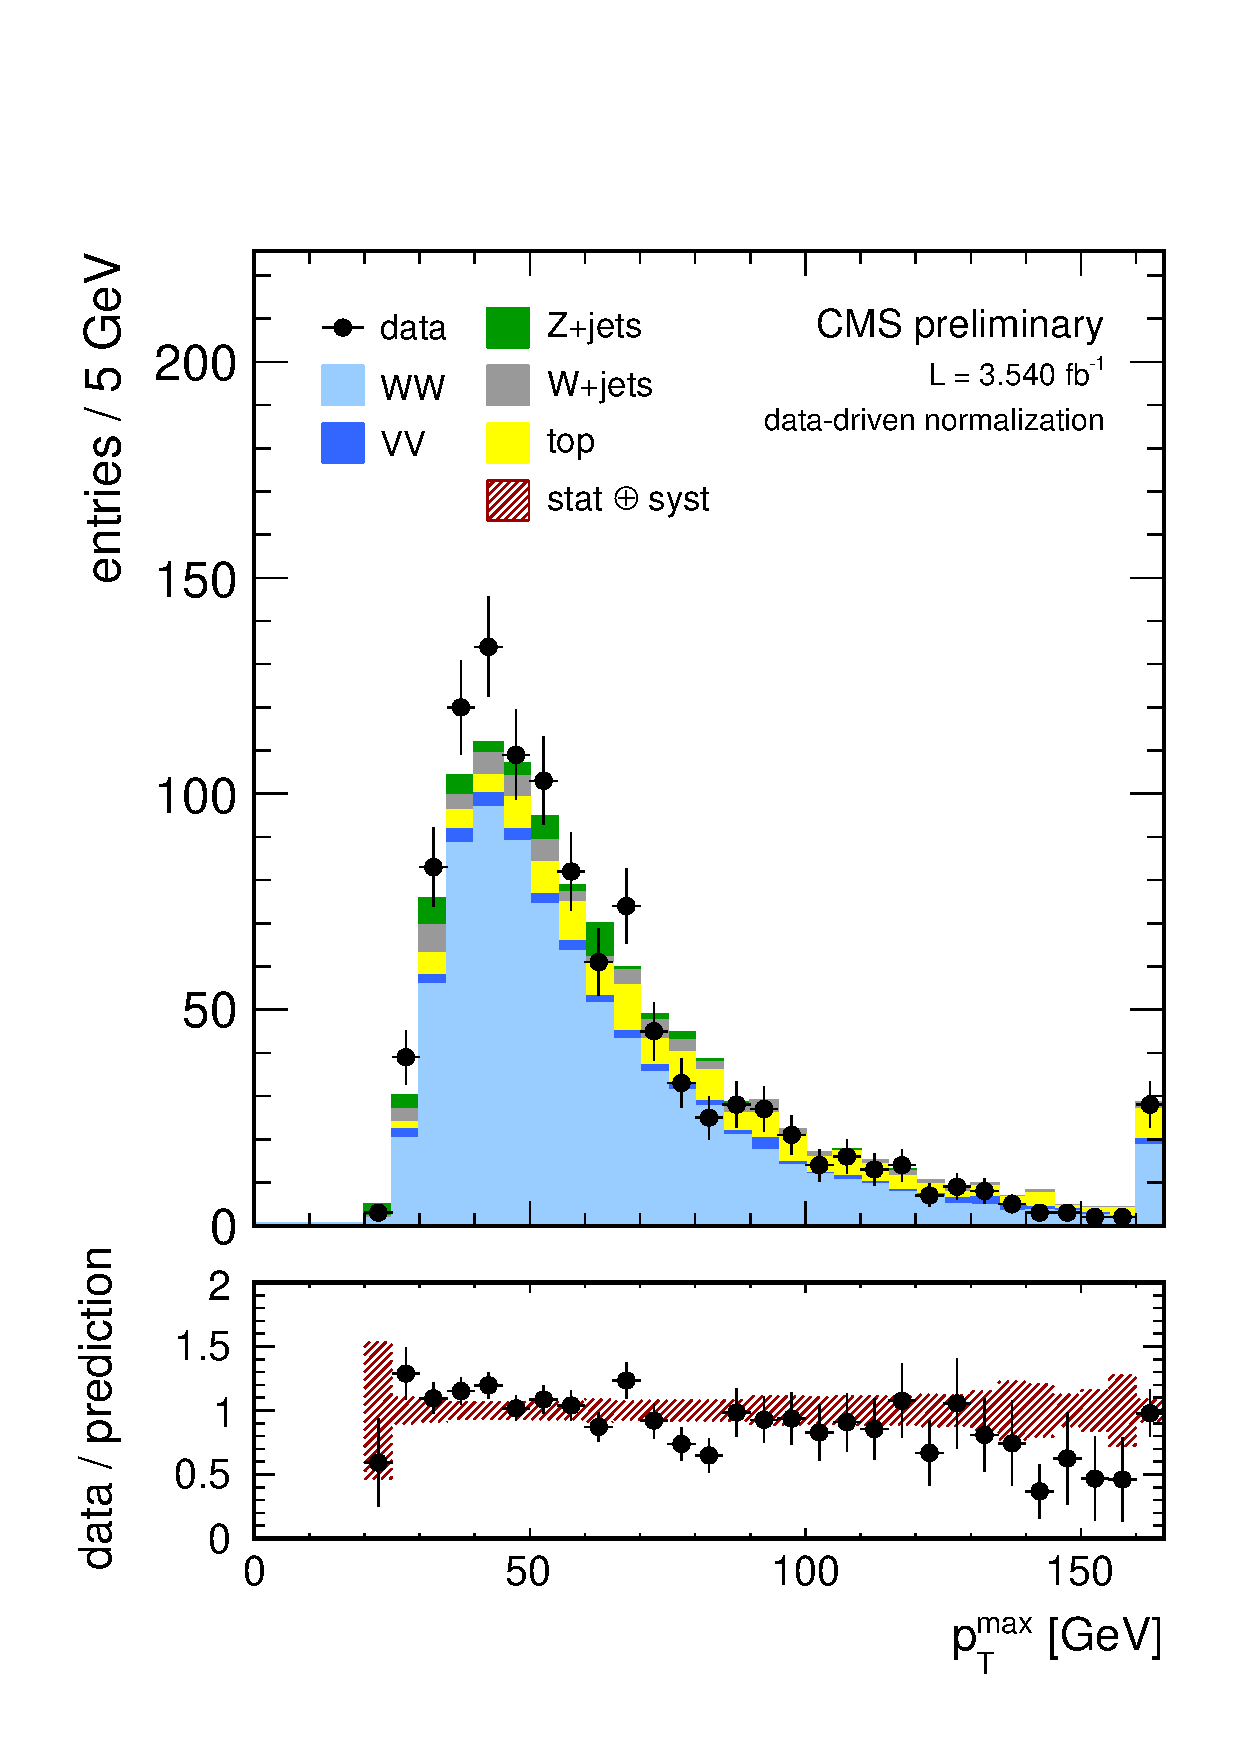
\includegraphics[width=0.45\textwidth]{figures/pt1} 
     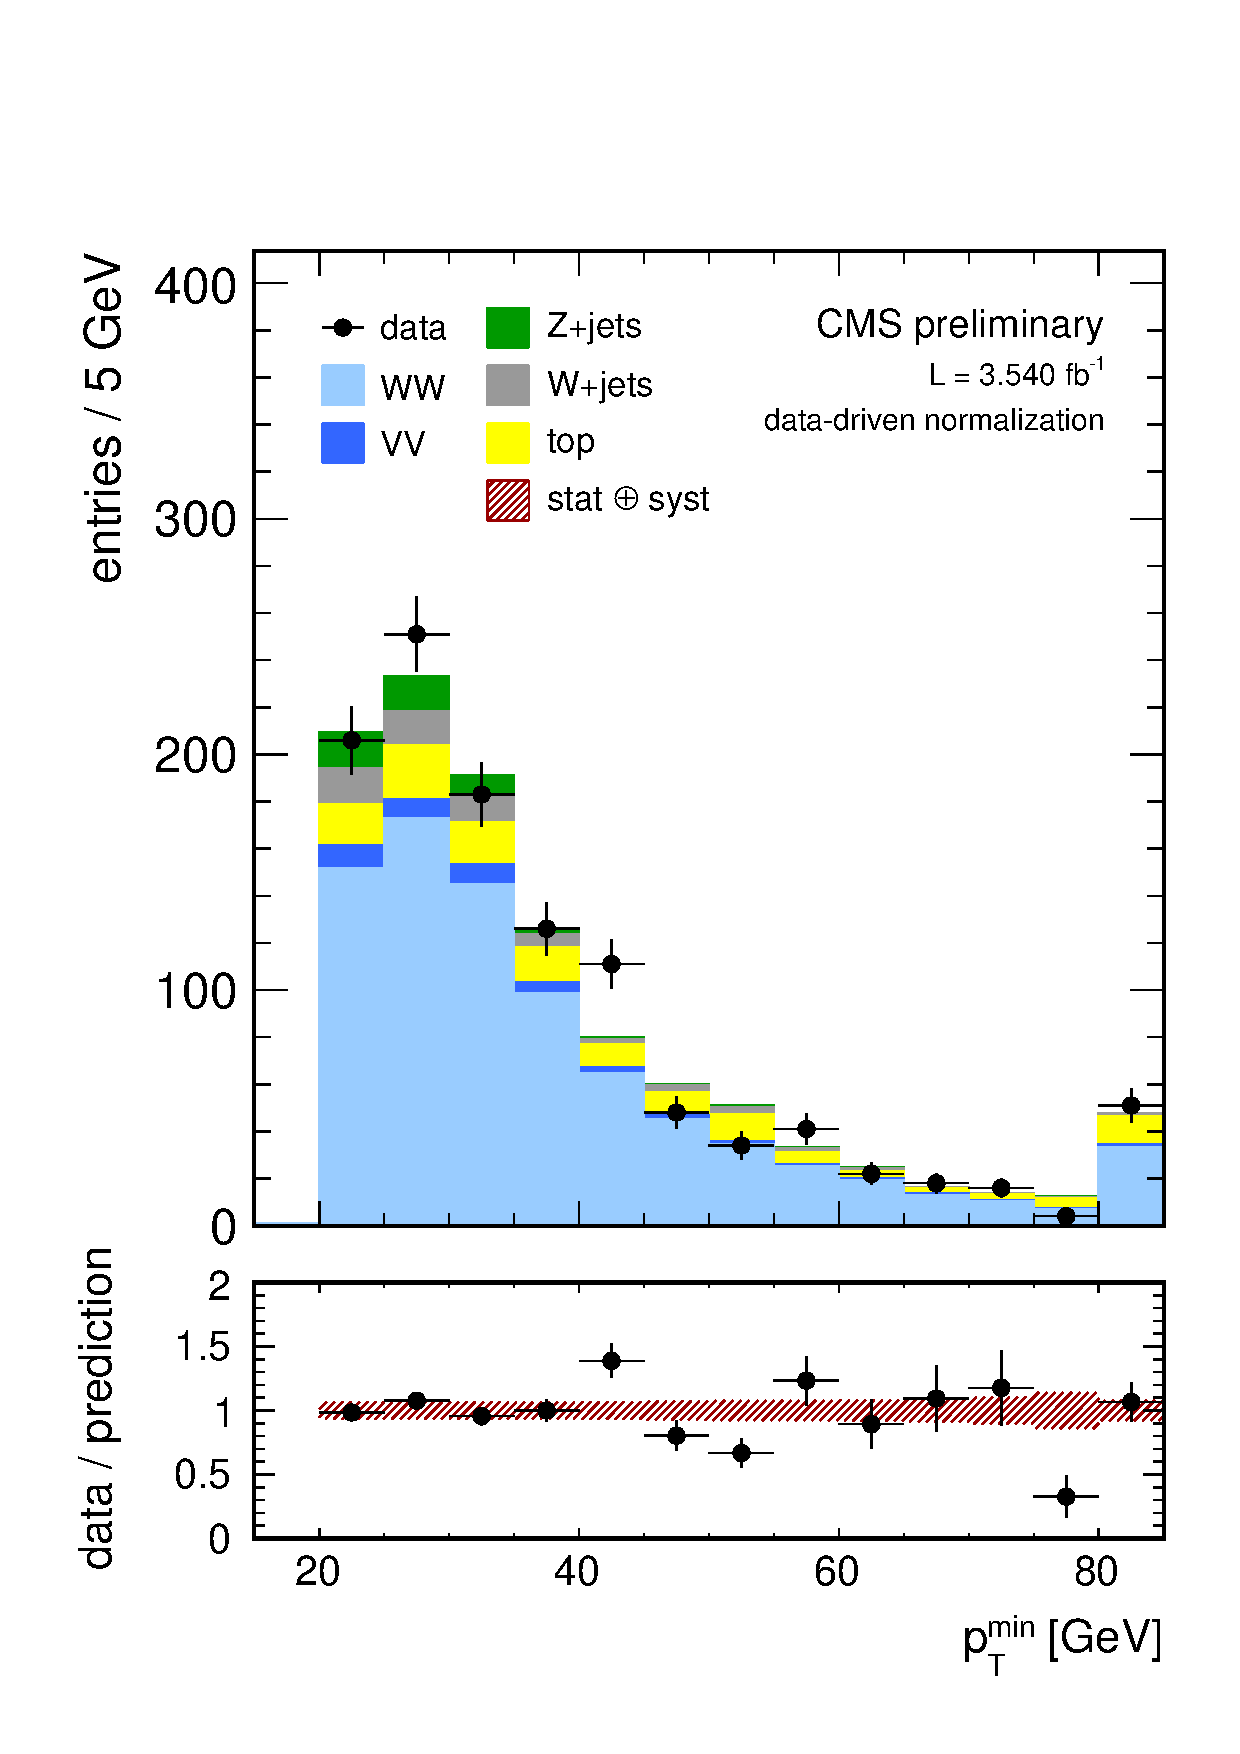
\includegraphics[width=0.45\textwidth]{figures/pt2}\\
     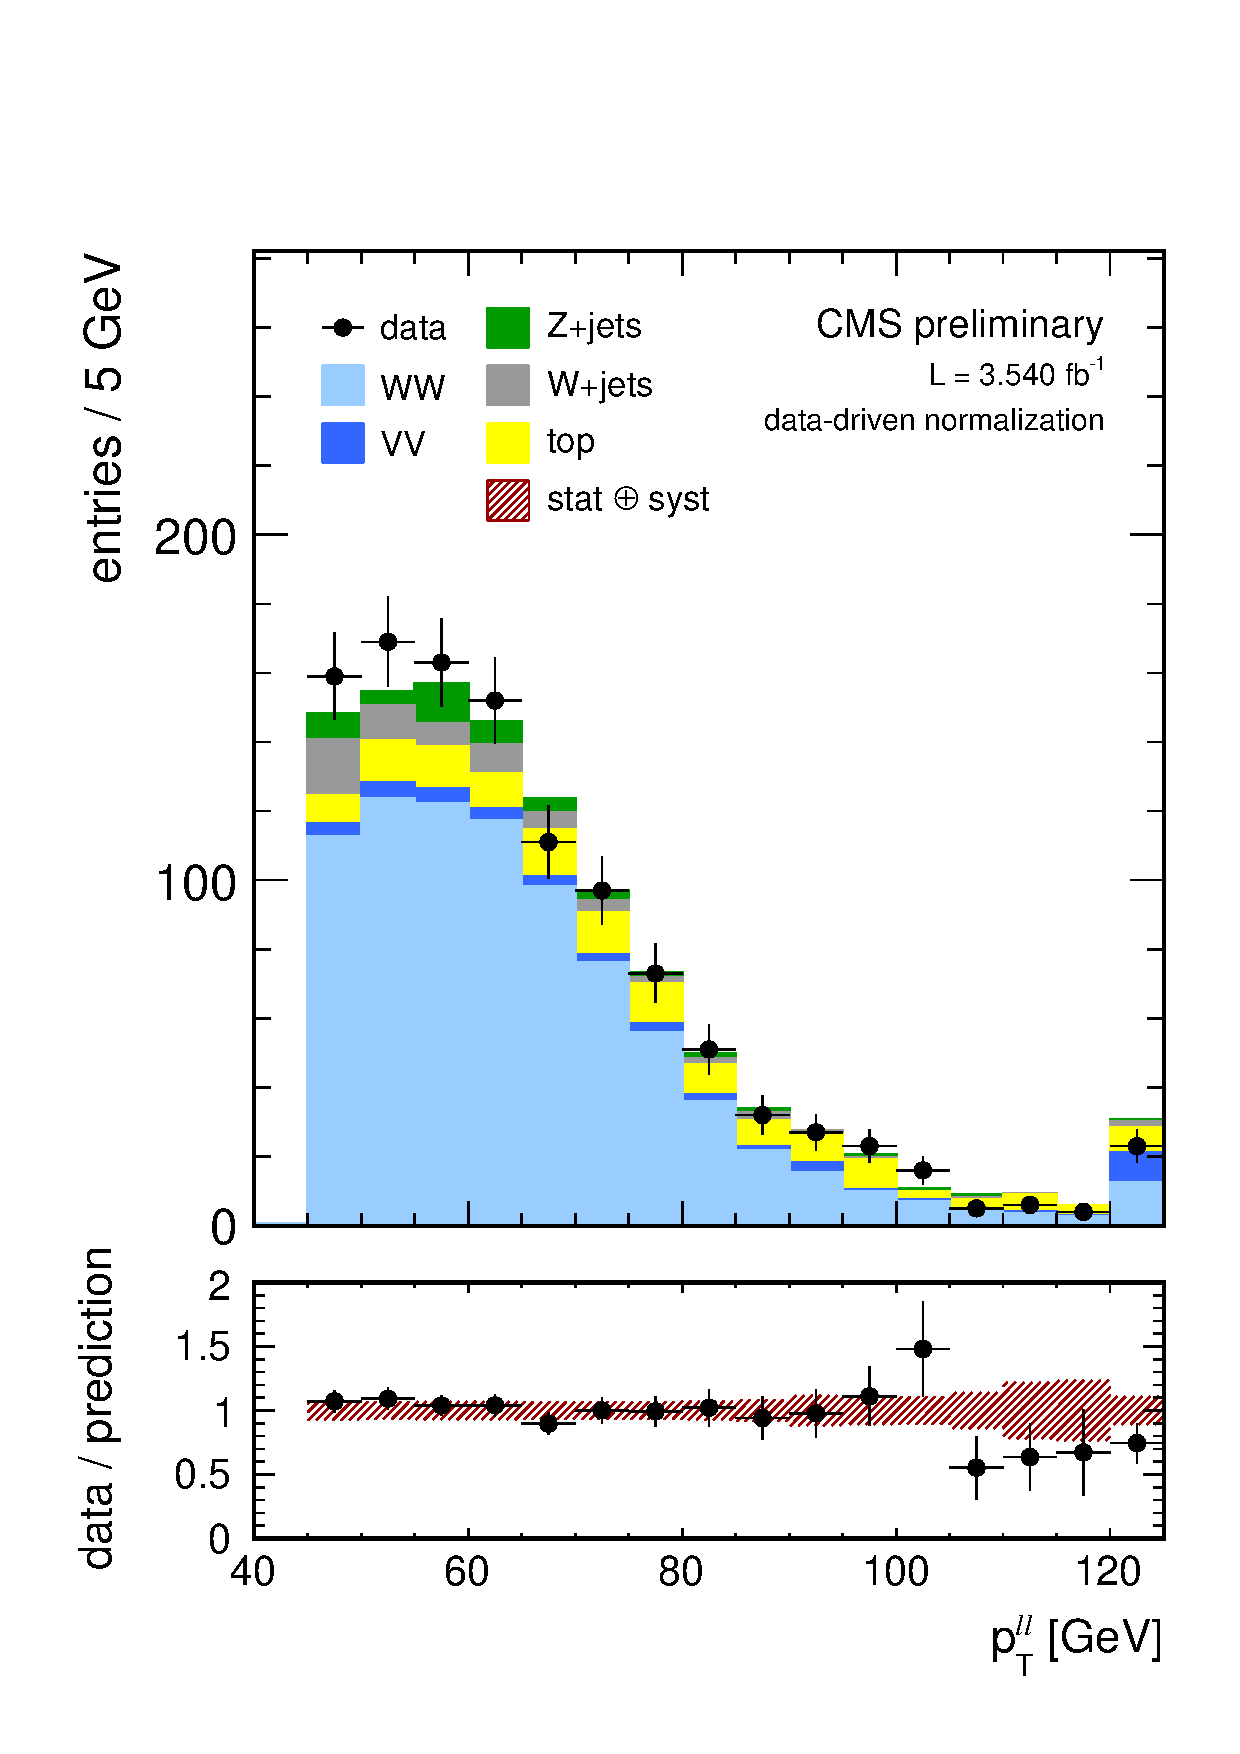
\includegraphics[width=0.45\textwidth]{figures/ptll} 
     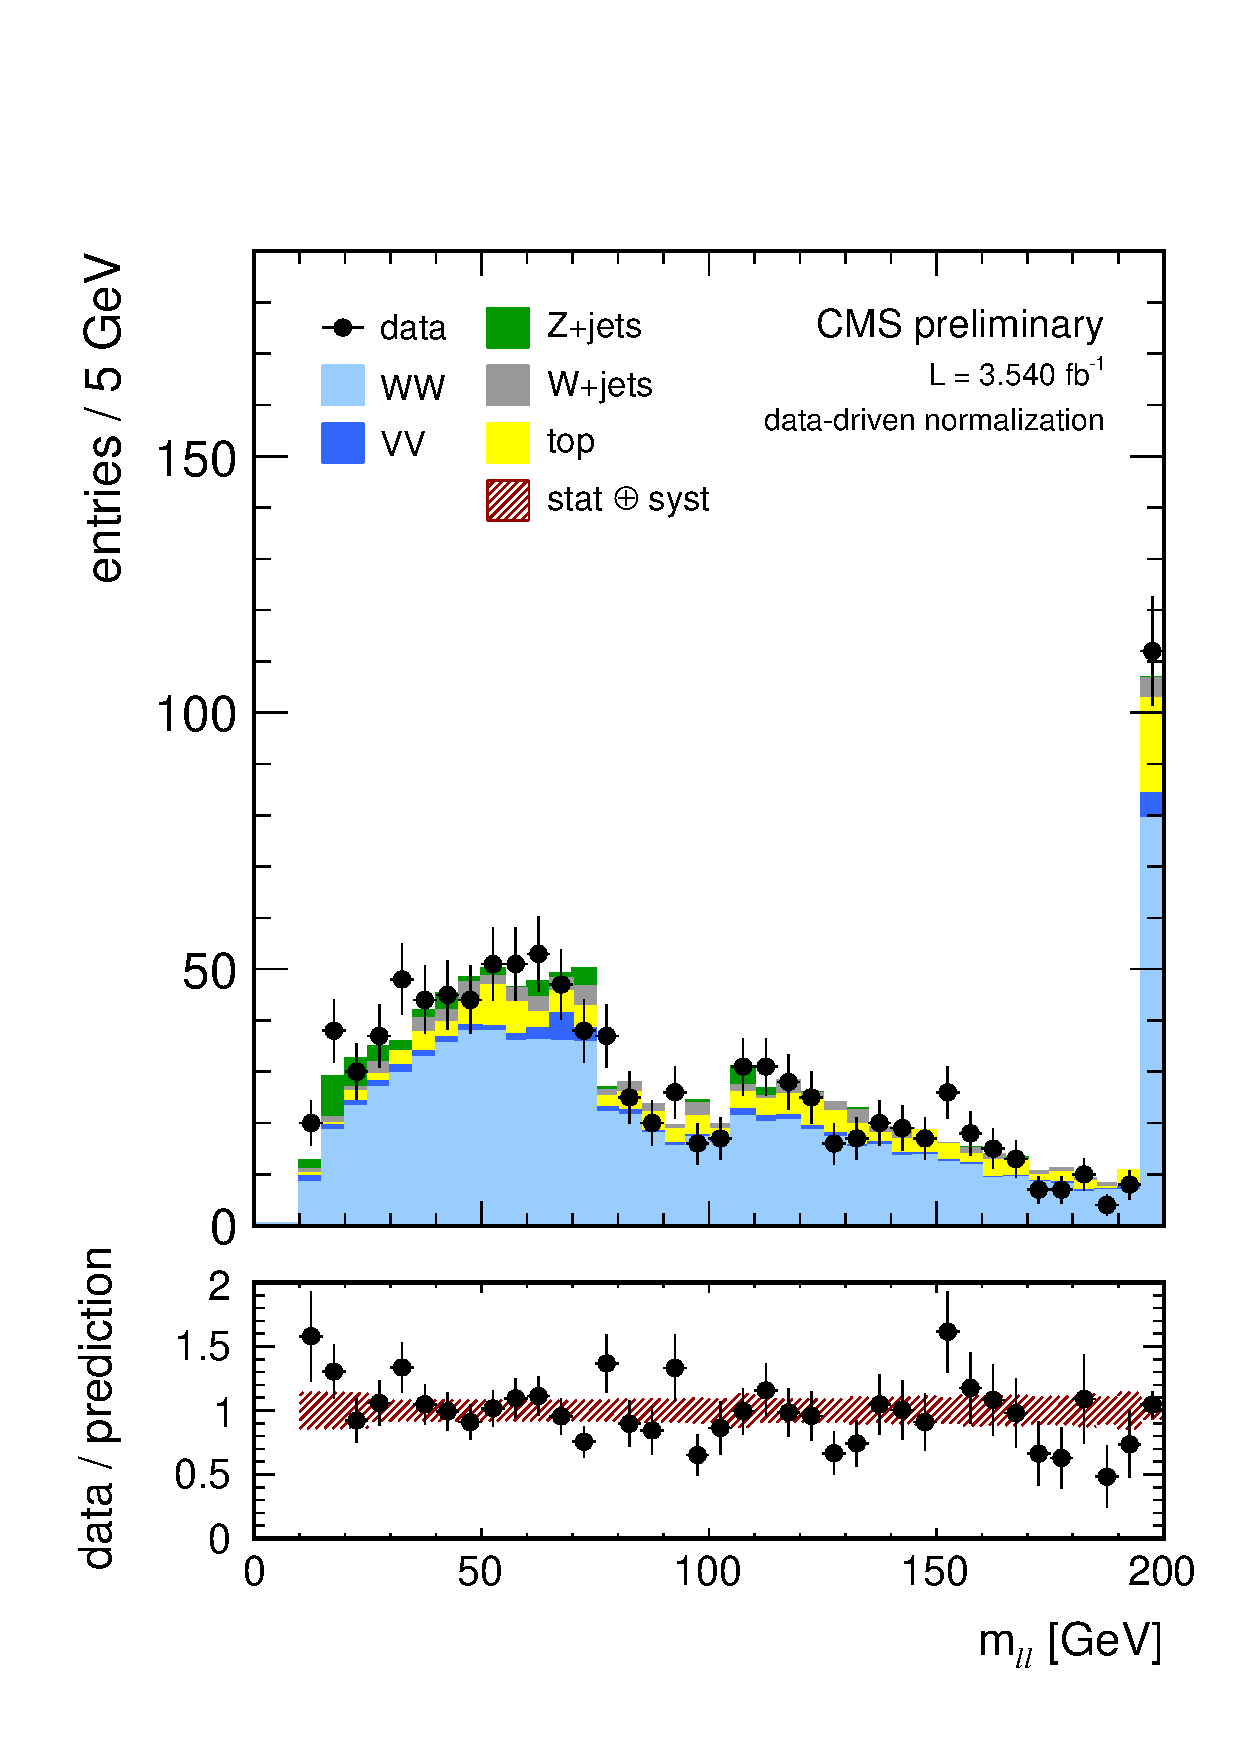
\includegraphics[width=0.45\textwidth]{figures/mll}\\

\end{tabular}
 \caption{Distributions of the leading lepton transverse momentum ($p_{\rm T}^{\rm max}$),
the trailing lepton transverse momentum ($p_{\rm T}^{\rm min}$), and
the dilepton transverse momentum ($\pt^{\ell\ell}$) and invariant mass ($m_{\ell\ell}$)
at the final selection level. The $\WW$ contribution is scaled to the CMS measurement
presented in this physics analysis summary.
All four channels (ee, $\mu\mu$, e$\mu$ and $\mu$e) are combined, and the uncertainty band corresponds
to the statistical and systematic uncertainties on the predicted yield.
 \label{fig:distributions}}
 \end{center}
\end{figure}
